%% fig_annihilator.tex   (generated by make_core.py; do not edit by hand)
%% H^{0,2} = wedge^2 H^{0,1} at n = 3 as the strict upper triangle of the 6 x 6 array: the two outer blocks are carried injectively by z -> z.omega, the n^2 = 9 mixed products form its kernel.
\documentclass[tikz,border=8pt]{standalone}
\usepackage{amsmath,amssymb}
\usetikzlibrary{arrows.meta,calc,decorations.pathreplacing}
%% palette.tex -- shared colour definitions for the figures
\definecolor{PInk}{RGB}{26,32,44}
\definecolor{PBlue}{RGB}{37,82,139}
\definecolor{PTeal}{RGB}{23,127,125}
\definecolor{POchre}{RGB}{193,138,44}
\definecolor{PClay}{RGB}{178,74,58}
\definecolor{PSlate}{RGB}{108,122,137}
\definecolor{PViolet}{RGB}{110,86,150}
\definecolor{WBlue}{RGB}{223,234,246}
\definecolor{WTeal}{RGB}{220,238,236}
\definecolor{WOchre}{RGB}{250,240,218}
\definecolor{WClay}{RGB}{247,229,224}
\definecolor{WSlate}{RGB}{238,241,244}
\definecolor{PMag}{RGB}{158,58,110}
\definecolor{PGrass}{RGB}{62,124,66}
\definecolor{PAmber}{RGB}{214,112,38}
\definecolor{PIndigo}{RGB}{58,64,140}
\definecolor{PRule}{RGB}{176,186,197}

%% shared macros so the standalone figures match the paper
\providecommand{\QQ}{\mathbb{Q}}
\providecommand{\ZZ}{\mathbb{Z}}
\providecommand{\RR}{\mathbb{R}}
\providecommand{\CC}{\mathbb{C}}
\providecommand{\PP}{\mathbb{P}}
\providecommand{\Kx}{K^{\times}}
\providecommand{\HW}{W}
\providecommand{\Nm}{\mathrm{N}}
\providecommand{\Hdg}{\mathrm{Hdg}}
\providecommand{\NS}{\mathrm{NS}}
\providecommand{\cA}{\mathcal{A}}
\providecommand{\cD}{\mathcal{D}}
\providecommand{\cF}{\mathcal{F}}
\providecommand{\cP}{\mathcal{P}}
\providecommand{\cO}{\mathcal{O}}
\providecommand{\cQ}{\mathcal{Q}}
\providecommand{\bbar}[1]{\overline{#1}}
\providecommand{\ch}{\operatorname{ch}}
\providecommand{\End}{\mathrm{End}}
\providecommand{\Ext}{\operatorname{Ext}}
\providecommand{\Supp}{\operatorname{Supp}}

\begin{document}
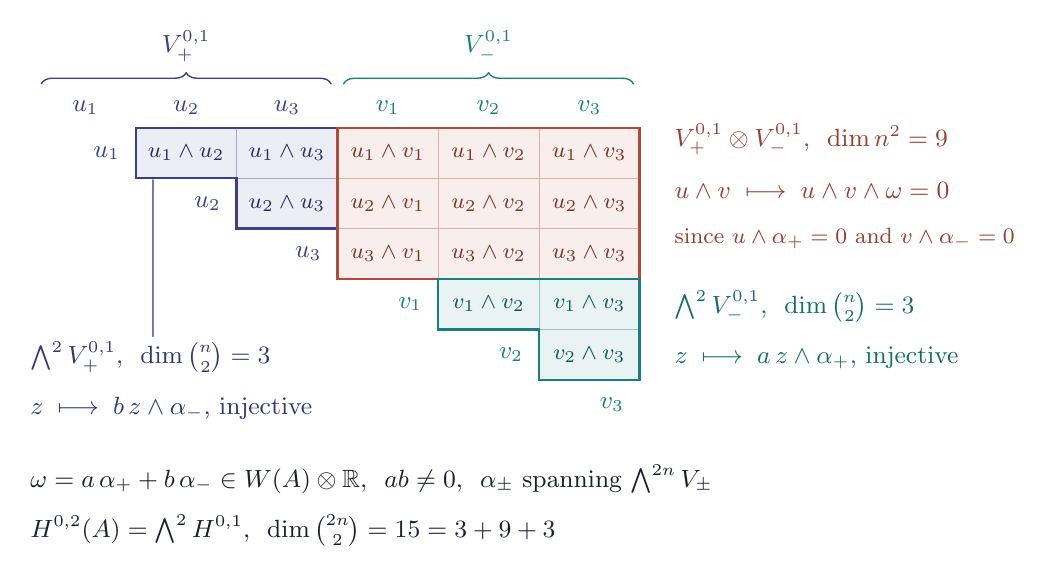
\begin{tikzpicture}[x=1cm,y=1cm,line join=round,line cap=round,
  font=\small,text=PInk,lbl/.style={inner sep=1pt}]
  \path[fill=PIndigo!9,draw=PIndigo!45,line width=0.3pt] (1.2800,0.0000) rectangle (2.5600,-0.6400);
  \path[fill=PIndigo!9,draw=PIndigo!45,line width=0.3pt] (2.5600,0.0000) rectangle (3.8400,-0.6400);
  \path[fill=PClay!9,draw=PClay!45,line width=0.3pt] (3.8400,0.0000) rectangle (5.1200,-0.6400);
  \path[fill=PClay!9,draw=PClay!45,line width=0.3pt] (5.1200,0.0000) rectangle (6.4000,-0.6400);
  \path[fill=PClay!9,draw=PClay!45,line width=0.3pt] (6.4000,0.0000) rectangle (7.6800,-0.6400);
  \path[fill=PIndigo!9,draw=PIndigo!45,line width=0.3pt] (2.5600,-0.6400) rectangle (3.8400,-1.2800);
  \path[fill=PClay!9,draw=PClay!45,line width=0.3pt] (3.8400,-0.6400) rectangle (5.1200,-1.2800);
  \path[fill=PClay!9,draw=PClay!45,line width=0.3pt] (5.1200,-0.6400) rectangle (6.4000,-1.2800);
  \path[fill=PClay!9,draw=PClay!45,line width=0.3pt] (6.4000,-0.6400) rectangle (7.6800,-1.2800);
  \path[fill=PClay!9,draw=PClay!45,line width=0.3pt] (3.8400,-1.2800) rectangle (5.1200,-1.9200);
  \path[fill=PClay!9,draw=PClay!45,line width=0.3pt] (5.1200,-1.2800) rectangle (6.4000,-1.9200);
  \path[fill=PClay!9,draw=PClay!45,line width=0.3pt] (6.4000,-1.2800) rectangle (7.6800,-1.9200);
  \path[fill=PTeal!9,draw=PTeal!45,line width=0.3pt] (5.1200,-1.9200) rectangle (6.4000,-2.5600);
  \path[fill=PTeal!9,draw=PTeal!45,line width=0.3pt] (6.4000,-1.9200) rectangle (7.6800,-2.5600);
  \path[fill=PTeal!9,draw=PTeal!45,line width=0.3pt] (6.4000,-2.5600) rectangle (7.6800,-3.2000);
  \draw[PIndigo,line width=0.9pt,line join=miter] (1.2800,0.0000) -- (3.8400,0.0000) -- (3.8400,-1.2800) -- (2.5600,-1.2800) -- (2.5600,-0.6400) -- (1.2800,-0.6400) -- cycle;
  \draw[PClay,line width=0.9pt,line join=miter] (3.8400,0.0000) rectangle (7.6800,-1.9200);
  \draw[PTeal,line width=0.9pt,line join=miter] (5.1200,-1.9200) -- (7.6800,-1.9200) -- (7.6800,-3.2000) -- (6.4000,-3.2000) -- (6.4000,-2.5600) -- (5.1200,-2.5600) -- cycle;
  \draw[PIndigo,line width=0.5pt,decorate,decoration={brace,amplitude=4pt}] (0.0800,0.5600) -- (3.7600,0.5600);
  \draw[PTeal,line width=0.5pt,decorate,decoration={brace,amplitude=4pt}] (3.9200,0.5600) -- (7.6000,0.5600);
  \draw[PIndigo!70,line width=0.45pt] (1.5000,-2.6500) -- (1.5000,-0.6600);
  \node[lbl,text=PIndigo!70!black,font=\footnotesize] at (1.9200,-0.3200) {$u_{1}\wedge u_{2}$};
  \node[lbl,text=PIndigo!70!black,font=\footnotesize] at (3.2000,-0.3200) {$u_{1}\wedge u_{3}$};
  \node[lbl,text=PClay!70!black,font=\footnotesize] at (4.4800,-0.3200) {$u_{1}\wedge v_{1}$};
  \node[lbl,text=PClay!70!black,font=\footnotesize] at (5.7600,-0.3200) {$u_{1}\wedge v_{2}$};
  \node[lbl,text=PClay!70!black,font=\footnotesize] at (7.0400,-0.3200) {$u_{1}\wedge v_{3}$};
  \node[lbl,text=PIndigo!70!black,font=\footnotesize] at (3.2000,-0.9600) {$u_{2}\wedge u_{3}$};
  \node[lbl,text=PClay!70!black,font=\footnotesize] at (4.4800,-0.9600) {$u_{2}\wedge v_{1}$};
  \node[lbl,text=PClay!70!black,font=\footnotesize] at (5.7600,-0.9600) {$u_{2}\wedge v_{2}$};
  \node[lbl,text=PClay!70!black,font=\footnotesize] at (7.0400,-0.9600) {$u_{2}\wedge v_{3}$};
  \node[lbl,text=PClay!70!black,font=\footnotesize] at (4.4800,-1.6000) {$u_{3}\wedge v_{1}$};
  \node[lbl,text=PClay!70!black,font=\footnotesize] at (5.7600,-1.6000) {$u_{3}\wedge v_{2}$};
  \node[lbl,text=PClay!70!black,font=\footnotesize] at (7.0400,-1.6000) {$u_{3}\wedge v_{3}$};
  \node[lbl,text=PTeal!70!black,font=\footnotesize] at (5.7600,-2.2400) {$v_{1}\wedge v_{2}$};
  \node[lbl,text=PTeal!70!black,font=\footnotesize] at (7.0400,-2.2400) {$v_{1}\wedge v_{3}$};
  \node[lbl,text=PTeal!70!black,font=\footnotesize] at (7.0400,-2.8800) {$v_{2}\wedge v_{3}$};
  \node[lbl,text=PIndigo] at (0.6400,0.2600) {$u_{1}$};
  \node[lbl,anchor=east,text=PIndigo] at (1.1200,-0.3200) {$u_{1}$};
  \node[lbl,text=PIndigo] at (1.9200,0.2600) {$u_{2}$};
  \node[lbl,anchor=east,text=PIndigo] at (2.4000,-0.9600) {$u_{2}$};
  \node[lbl,text=PIndigo] at (3.2000,0.2600) {$u_{3}$};
  \node[lbl,anchor=east,text=PIndigo] at (3.6800,-1.6000) {$u_{3}$};
  \node[lbl,text=PTeal] at (4.4800,0.2600) {$v_{1}$};
  \node[lbl,anchor=east,text=PTeal] at (4.9600,-2.2400) {$v_{1}$};
  \node[lbl,text=PTeal] at (5.7600,0.2600) {$v_{2}$};
  \node[lbl,anchor=east,text=PTeal] at (6.2400,-2.8800) {$v_{2}$};
  \node[lbl,text=PTeal] at (7.0400,0.2600) {$v_{3}$};
  \node[lbl,anchor=east,text=PTeal] at (7.5200,-3.5200) {$v_{3}$};
  \node[lbl,text=PIndigo] at (1.9200,1.0400) {$V_{+}^{0,1}$};
  \node[lbl,text=PTeal] at (5.7600,1.0400) {$V_{-}^{0,1}$};
  \node[lbl,anchor=west,text=PClay!85!black] at (8.0800,-0.1500) {$V_{+}^{0,1}\otimes V_{-}^{0,1}$,\ \ $\dim n^{2}=9$};
  \node[lbl,anchor=west,text=PClay!85!black] at (8.0800,-0.8000) {$u\wedge v\;\longmapsto\;u\wedge v\wedge\omega=0$};
  \node[lbl,anchor=west,text=PClay!85!black,font=\footnotesize] at (8.0800,-1.4000) {since $u\wedge\alpha_{+}=0$ and $v\wedge\alpha_{-}=0$};
  \node[lbl,anchor=west,text=PTeal!85!black] at (8.0800,-2.2700) {$\bigwedge^{2}V_{-}^{0,1}$,\ \ $\dim\binom{n}{2}=3$};
  \node[lbl,anchor=west,text=PTeal!85!black] at (8.0800,-2.9200) {$z\;\longmapsto\;a\,z\wedge\alpha_{+}$, injective};
  \node[lbl,anchor=west,text=PIndigo!85!black] at (-0.1000,-2.9100) {$\bigwedge^{2}V_{+}^{0,1}$,\ \ $\dim\binom{n}{2}=3$};
  \node[lbl,anchor=west,text=PIndigo!85!black] at (-0.1000,-3.5600) {$z\;\longmapsto\;b\,z\wedge\alpha_{-}$, injective};
  \node[lbl,anchor=west,text=PInk] at (-0.1000,-4.4600) {$\omega=a\,\alpha_{+}+b\,\alpha_{-}\in\HW(A)\otimes\RR$,\ \ $ab\neq0$,\ \ $\alpha_{\pm}$ spanning $\bigwedge^{2n}V_{\pm}$};
  \node[lbl,anchor=west,text=PInk] at (-0.1000,-5.1100) {$H^{0,2}(A)=\bigwedge^{2}H^{0,1}$,\ \ $\dim\binom{2n}{2}=15=3+9+3$};
\end{tikzpicture}
\end{document}
